% --------------------------------------------------
% 
% This chapter is for Tristomo
% 
% --------------------------------------------------

\chapter{
    Studying real-world microbial communities
}
\label{cha:swamp}


% AFOULOPAPER
\section{
   Deciphering the functional potential of a hypersaline marsh microbial mat community
}
\label{publ:tristomo-ecology}

\textbf{Status:} \\ 
   Pavloudi C, Zafeiropoulos H, 
   Deciphering the functional potential of a hypersaline marsh microbial mat community.\\
   Under review in FEMS Microbiology Ecology. \\ 
   Shared co-authorship and correspondance.


\subsection{Abstract}

   Microbial mats are vertically stratified communities of microorganisms characterised by 
   pronounced physiochemical gradients allowing for high species diversity 
   and a wide range of metabolic capabilities. 
   High Throughput Sequencing has the potential to reveal the biodiversity and function of such ecosystems 
   in the cycling of elements and organic matter recycling.

   The present study combines 16S rRNA amplicon sequencing and shotgun metagenomics 
   on sediments and microbial mats from a hypersaline marsh in Tristomo bay 
   (Karpathos, Greece). 
   Sampling was conducted in July 2018 and November 2019. 
   Samples were collected from the microbial mats and the deeper sediment; 
   orange and pink microbial aggregates observed in the water overlying the 
   sediment were also collected, as well as sediment samples with no apparent layering.

   Metagenomic assembly and binning in the sample level, revealed 250 bacterial 
   and 39 archaeal metagenome-assembled genomes, 
   with completeness estimates higher than 70\%  and contamination less than 5%. 
   Halobacteria and Bacteroidetes were among the most abundant taxa in the microbial mats. 
   Photosynthesis was most likely performed by purple sulphur and non-sulphur bacteria. 
   
   Overall, both the sequencing methodologies seemed to result in similar 
   taxonomic compositions. 
   All samples had the functional capacity for sulphate reduction, 
   dissimilatory arsenic reduction and conversion of pyruvate to oxaloacetate. 


% AFOULOPAPER INTRODUCTION
\subsection{Introduction}
\label{swamp:intro}

   Microbial mats are vertically stratified communities of functional groups of microorganisms embedded in an organic matrix, 
   which may also contain minerals such as silicates and carbonates 
   \citep{stal_cyanobacterial_2012, bolhuis_molecular_2014, prieto-barajas_microbial_2018}. 
   They grow on a solid substrate (e.g. sand) and the vast majority of microbial mats utilise inorganic carbon as carbon source, 
   hence they are autotrophic~\citep{bolhuis_molecular_2014}. 
   Microbial mats are characterised by pronounced physiochemical gradients which allow for the presence of high species diversity, 
   encompassing a wide range of metabolic capabilities; 
   thus, mats are ideal models to study a whole ecosystem~\citep{al-thani_community_2014} and are considered as 
   natural laboratories~\citep{villanueva_analysis_2007}. 
   These physicochemical gradients provide microenvironments for various microbial functional groups, which exhibit 
   a certain physiology with which they fulfil a specific function~\citep{van_gemerden_microbial_1993}. 
   
   Microbial mats comprise millions of microorganisms belonging to different species which are embedded in a matrix of 
   extracellular polymers (EPS) and exchange signals and nutrients, 
   thus enabling a flow of resources and energy for the survival of the overall community 
   \citep{ruvindy_unravelling_2016, prieto-barajas_microbial_2018}. 
   The role of microbial mats has been vital throughout Earth's history since they produced and released reduced gases, 
   e.g. O$_2$, H$_2$, CH$_4$, in the early earth's atmosphere \citep{hoehler_role_2001}. 
   In addition, they constitute the first ecosystems, along with stromatolites 
   \citep{santoyo_unveiling_2021}, 
   and probably are the oldest structured ecosystems on earth~\citep{van_gemerden_microbial_1993}.

   Regardless of the vertical structure, marine microbial mats are comprised of four main functional groups: 
   i) oxygenic phototrophs (CYN) (primarily Cyanobacteria), 
   ii) aerobic heterotrophic bacteria (HET), 
   iii) sulphate-reducing bacteria (SRB) and 
   iv) sulphide-oxidising bacteria (SOB)~\citep{visscher_microbial_2005}. 
   Microbial mats function as a consortium where coupling of biogeochemical cycles and processes occurs~\citep{paerl_cyanobacterialbacterial_2000}, 
   allowing the products of the metabolism of one group to be available and used by another~\citep{santoyo_unveiling_2021}. 
   In addition, the metabolic rates of mat microorganisms are so high that the community production per unit mass competes with that of rainforests
   \citep{jorgensen_diffusion_1994, krumbein_fossil_2003}. 

   Microbial mats can be distinguished in six categories 
   \citep{bolhuis_molecular_2014, prieto-barajas_microbial_2018}: 
   i) intertidal or coastal, 
   ii) hypersaline, 
   iii) hot spring, 
   iv) mats in oligotrophic environments, 
   v) psychrophile and vi) acid microbial mats. 
   Intertidal mats are formed on beaches with low slopes and fine sandy sediments~\citep{stal_cyanobacterial_2012} 
   and they experience strong salinity fluctuations, large temperature changes~\citep{bolhuis_molecular_2014}
   and irregular floods~\citep{prieto-barajas_microbial_2018}. 
   On the other hand, hypersaline microbial mats are found in natural occurring salt lakes and man-made salterns~\citep{bolhuis_molecular_2014} and are exposed to salinities up to 
   the crystallisation point of halite~\citep{jorgensen_diffusion_1994}, 
   high temperatures and high solar radiation~\citep{bolhuis_molecular_2014}. 
   
   The present study was conducted in the Tristomo marsh in the island of Karpathos (Aegean Sea, Greece) (Figure~\ref{fig:karpathos-marsh} A). 
   The marsh is located at the northern end of Karpathos. 
   The study area is included in the Natura 2000 network (site GR4210003) and also in the catalogue of small island wetlands 
   (Government Gazette Issue on Compulsory Expropriations and City-Planning 229/19.6.2012) with the code Y421KAR001 (total area: 1.9 ha) (Figure~\ref{fig:karpathos-marsh} B). 
   It is a seasonal brackish water marsh formed at the edge of a small plain where a seasonal stream ends, 
   characterised as an intertidal marsh (type H) according to the \href{https://www.ramsar.org/about/the-convention-on-wetlands-and-its-mission}{Ramsar convention}. 
   In the past, it probably occupied a larger area and was connected to the stream. 
   Most of the area is fenced with dry stones that used to be cultivated systematically. 
   Today crops exist in only a small part and there is livestock grazing around the marsh. 
   On the coastal front, the cobbled beach is full of garbage carried by the waves. 
   Freshwater enters the marsh from the precipitation and drainage basin, while the wetland interacts mainly with the sea through the waves 
   but also underground~\citep{wwf_greece_inventory_2022}. 
   Due to the close proximity of the marsh with the sea, it occasionally receives saline water, therefore could be characterised as intertidal; 
   however, crystallised salt forms an upper layer above the actual microbial mat, something that is observed in hypersaline mats (Figure~\ref{fig:karpathos-marsh} C and D). 
   High Throughput Sequencing (HTS) technologies and methods have been widely used to study real-world microbial communities. 
   They have enabled the study of ecosystems with no prior knowledge of the resident species, uncovering unknown and uncultivated strains~\citep{hedlund_impact_2014}. 
   Metabarcoding studies are common, well-established and less computationally demanding than shotgun metagenomics~\citep{bell_comparing_2021}. 
   However, taxonomic biases may arise from differential efficiency of PCR primer pairing in different species~\citep{van_der_loos_biases_2021}
   while the short barcoding sequences may limit the resolution. 
   On the other hand, shotgun metagenomics by obtaining information from random sampling of virtually all genomic regions, 
   enables profiling up to the level of strains~\citep{clooney_comparing_2016, segata_road_2018, davila-ramos_review_2019}. 
   Therefore, microbiome metabolic functions and entire biochemical pathways that occur in a sample can be explored after processing 
   the metagenomic information~\citep{sharpton_introduction_2014}. 

   \begin{figure}[!htbp]
      \centering
      \includegraphics[width=0.85\columnwidth]{figures/karpathos-swamp.png}
      \caption[Tristomo marsh in Karpathos overview]{
         A) Location of Karpathos island (red pin) in the south east of the Aegean Sea, 
         B) satellite image of Tristomo bay and the Tristomo marsh (red pin), 
         C) overview of the marsh in July 2018, 
         D) overview of the marsh in July 2018, where orange aggregates floating in the water are shown and 
         E) a sediment core from 2018 including salt crust, microbial mat, sediment and an orange aggregate. 
         (Map data: ©2022 Google Earth).
      }
      \label{fig:karpathos-marsh}
   \end{figure}   



   Over the recent years, HTS approaches have been used to study the taxonomic and the functional 
   profiles of the microbial communities present in microbial mats 
   \citep{chen_discovery_2020, wong_microbial_2020, kindler_genome-resolved_2022}. 
   Several novel high-level taxa have been discovered, e.g. Zixibacterial order GN15~\citep{wong_microbial_2020}, 
   and a better understanding on both their adaptive responses in such environments has been established. 
   On top of that, further insight on the mechanisms governing such assemblages has been gained, e.g. the role of photoheterotrophy 
   \citep{kindler_genome-resolved_2022}. 
   The aim of the present study was to identify the microbial communities present in samples from the 
   hypersaline Tristomo marsh, as well as their functional and metabolic capabilities.


% AFOULOPAPER METHODS
\subsection{Methods}
\label{swamp:methods}

\subsubsection*{Sample collection}

   Samples were collected in July 2018 and November 2019 from the Tristomo marsh (Figure~\ref{fig:karpathos-marsh}). 
   Details on the sample collection are given in Table~\ref{table:sampling}. 
   Sediment samples were collected using cylindrical sampling corers (internal sampling surface 15.90 square centimetres) (Figure~\ref{fig:karpathos-marsh}.E). 
   In the cases where microbial mat layers were clearly observed (July 2018), the top layer was collected separately from the bottom layer. 
   In addition, microbial aggregates observed floating in the marsh were also collected. 
   In the cases where microbial mat layers were not clearly formed (November 2019), there was no slicing during sample collection. 
   In November, samples were collected from three different locations in the marsh, distinguished by the colour of the sediment’s upper layer (black, purple and orange). 

   \begin{sidewaystable}
      \small
      \begin{tabular}{llllllll}
      \toprule
      \textbf{Sample} & \textbf{Type} & \textbf{Date} & \textbf{\begin{tabular}[c]{@{}l@{}}16S rRNA \\ accession number\end{tabular}} & \textbf{\begin{tabular}[c]{@{}l@{}}shotgun accession \\ number (lane 1)\end{tabular}} & \textbf{\begin{tabular}[c]{@{}l@{}}shotgun accession \\ number (lane 2)\end{tabular}} & \textbf{latitude} & \textbf{longitude} \\
      \toprule
      Elos01 & top sediment layer & 8/7/2018 & ERR9657902 & ERR6290772 & ERR6290778 & 35.81936 & 27.20984 \\
      Elos02 & bottom sediment layer & 8/7/2018 & ERR9657903 & ERR6290773 & ERR6290779 & 35.81936 & 27.20984 \\
      Elos03 & orange aggregate & 8/7/2018 & ERR9657904 & ERR6290774 & ERR6290780 & 35.81936 & 27.20984 \\
      Elos04 & top sediment layer & 13/7/2018 & ERR9657905 &  &  & 35.81936 & 27.20984 \\
      Elos05 & bottom sediment layer & 13/7/2018 & ERR9657906 &  &  & 35.81936 & 27.20984 \\
      Elos06 & orange aggregate & 13/7/2018 & ERR9657907 &  &  & 35.81936 & 27.20984 \\
      Elos07 & pink aggregate & 13/7/2018 & ERR9657908 & ERR6290775 & ERR6290781 & 35.81936 & 27.20984 \\
      Elos08 & top sediment layer & 9/7/2018 & ERR9657909 &  &  & 35.81936 & 27.20984 \\
      Elos09 & bottom sediment layer & 9/7/2018 & ERR9657910 &  &  & 35.81936 & 27.20984 \\
      Elos10 & \begin{tabular}[c]{@{}l@{}}sediment (combined \\ layers, black upper layer)\end{tabular} & 12/11/2019 & ERR9657898 & ERR6290776 & ERR6290782 & 35.81962 & 27.2102 \\
      Elos11 & \begin{tabular}[c]{@{}l@{}}sediment (combined \\ layers, black upper layer)\end{tabular} & 12/11/2019 & ERR9657899 &  &  & 35.81962 & 27.2102 \\
      Elos12 & \begin{tabular}[c]{@{}l@{}}sediment (combined \\ layers, orange upper layer)\end{tabular} & 12/11/2019 & ERR9657900 & ERR6290777 & ERR6290783 & 35.81942 & 27.21007 \\
      Elos13 & \begin{tabular}[c]{@{}l@{}}sediment (combined \\ layers, purple upper layer)\end{tabular} & 12/11/2019 & ERR9657901 &  &  & 35.81943 & 27.20998
      \end{tabular}
      \caption[Details on Karpathos marsh sample collection.]{Details on Karpathos marsh sample collection.}
      \label{table:sampling}

   \end{sidewaystable}   


   Samples were placed in 50 ml falcon tubes (Sarstedt, Nümbrecht, Germany) and were stored at −20 °C, until further processing in the laboratory. 
   Upon return to the laboratory, they were used for molecular analysis, i.e. DNA extractions, as well as for the measurement of the Particulate Organic Carbon (POC) 
   and chloroplast pigments concentration (chlorophyll-a, phaeopigments and chloroplastic pigment equivalents (CPE)). 
   For the latter, the samples were processed at the \href{https://imbbc.hcmr.gr/infrastructures/facilitiesimbbc/environmental-chemistry-microbiology-labs/}{Environmental Chemistry Lab}
   of the IMBBC (HCMR), based on standard techniques \citep{yentsch_method_1963, hedges_carbon_1984}. 
   Water temperature and dissolved oxygen concentration were measured in the water overlaying the sediments by means of a portable multi-parameter (WTW Multi 3420 SET G). 
   Salinity was also measured with the portable multi-parameter but after dilution of samples with dH2O since the initial measurement was out of limits (TetraCon® 925 sensor range: 0 - 70). 
   Sampling was conducted under authorization from the relevant licensing authority (Directorate General for the Protection and Development of Forests and the Rural Environment, Directorate of Forest Management) of the Ministry of Environment and Energy. 
   Additional authorization was also provided from the Management Agency of Dodecanese Protected Areas. 


   \begin{figure}[!htbp]
      \centering
      \includegraphics[width=0.98\columnwidth]{figures/karpathos_16S_phyla.png}
      \caption[Tristomo marsh in Karpathos overview]{
         Bar chart showing the abundances of the main microbial taxa, at the phylum level, at each sample, based on the 16S rRNA amplicon sequencing. 
      }
      \label{fig:karpathos-16S}
   \end{figure}   


\subsubsection*{DNA extraction, PCR amplification and 16S rRNA sequencing}

   DNA was extracted as in \citep{henckel_molecular_1999} and \citep{lueders_enhanced_2004}. 
   Approximately 0.7 g of wet sediment were added to a 2-ml screw-cap vial, prefilled with ~0.7 g of 0.1 mm (diameter) zirconia/silica beads (11079101z, BioSpec, USA). 
   The vials were filled with 750 μl of 120 mM NaPO4 buffer (pH 8) and 250 μl TNS solution (500 mM Tris-HCl pH 8, 100 mM NaCl, 10 \% SDS (w/v)) and placed horizontally in a vortex for 10 minutes at maximum speed. 
   Immediately after that the vials were centrifuged for 10 min at 20,800 rcf and 4 °C and the supernatants were transferred to new 2-ml vials. 
   One volume of phenol/chloroform/isoamylalcohol (P/C/I; 25:24:1; pH 8; Carl-Roth, Karlsruhe, Germany) was added to the aqueous supernatant. 
   Vials were vigorously shaken for 20 s and centrifuged for 5 min at 20,800 rcf and 4 °C. 
   Supernatants were transferred to new 2-ml vials, and one volume of chloroform/isoamylalcohol (C/I; 24:1; Carl-Roth) was added. 
   Vials were again vigorously shaken for 20 s and then centrifuged for 5 min at 20,800 rcf and 4 °C. 
   Supernatants were transferred to new 2-ml vials and C/I extraction was repeated to successfully remove all phenol remnants. 
   Supernatants were transferred to new 2-ml vials and 1.5 ml of polyethylene glycol (30 \% (w/v) polyethylene glycol 6000 in 1.6 M NaCl) was added to precipitate nucleic acids and the vials were centrifuged for 90 min at 20,800 rcf and 4 °C. 
   Supernatants were discarded and the pellets were washed with 1 ml 70\% ethanol (4 °C) and centrifuged for 30 min. 
   Supernatants were again discarded, pellets were left for air drying (~5 min) to remove leftover ethanol and resuspended with 50 μl 10mM Tris. 
   PCR amplification, library preparation and MiSeq sequencing was performed as in \citep{pavloudi2017sediment}. 
   The PCR negative control sample (blank) was also sequenced, so that possible contamination during the library preparation could be assessed. 
   The raw sequence reads were processed with PEMA (version 2.1.4) \citep{zafeiropoulos2020pema} using VSEARCH for the creation of OTUs. 
   Taxonomic assignment was performed with the SILVA database (version 132) \citep{quast_silva_2013}. 
   The detailed parameters of the PEMA processing are given in Supplementary File 1. 
   The phyloseq (version 1.36) \citep{mcmurdie2013phyloseq}, vegan (version  2.5.7) \citep{oksanen_vegan_2020} and ggplot2 (version 3.3.5) \citep{wickham2016package} 
   packages were used in R (version 4.1.1) (R Core Team 2021) for the creation of barcharts, for the nMDS and PERMANOVA, variation partitioning analysis, db-RDA and mantel test. 
   The scripts of Steinberger (2020) \citep{steinberger_asteinberger9seq_scripts_2020} were used for the simper and the Kruskal-Wallis tests. 


\subsubsection*{Shotgun metagenomics sequencing}

   Six samples were selected for shotgun sequencing (Elos01, Elos02, Elos03, Elos07, Elos10 and Elos12). 
   Sample preparation was performed using the Nextera$^{TM}$ DNA Flex Tagmentation and sequencing was done at two lanes of a HiSeq 4000 (2x150bp) at the Norwegian Sequencing Centre (NSC). 
   All the raw sequence files of this study (both 16S rRNA and shotgun metagenomes) were submitted to the European Nucleotide Archive (ENA) \citep{cummins_european_2022} with the study accession number PRJEB46254 
   (available at: \\ \href{http://www.ebi.ac.uk/ena/data/view/PRJEB46254}{http://www.ebi.ac.uk/ena/data/view/PRJEB46254}).


\subsubsection*{Assembly and binning}

   Since the samples were sequenced in two lanes, the fastq files of each sample were concatenated before proceeding with the analyses. 
   Metagenome raw reads were processed with the \texttt{MetaWRAP} workflow (version 1.3.2)~\citep{uritskiy_metawrapflexible_2018}. 
   Reads were trimmed and qualified using \texttt{Trim Galore} (version 0.5.0)~\citep{krueger_trim_2022}, which is a wrapper around \texttt{Cutadapt} (version 1.18)~\citep{martin_cutadapt_2011} and \texttt{FastQC}. 
   The clean reads were concatenated and their co-assembly was implemented through the corresponding \texttt{MetaWRAP} module, using MEGAHIT v1.1.3. 
   The quality of the co-assembly was evaluated using \texttt{QUAST}~\citep{gurevich_quast_2013} 
   (see \href{https://github.com/hariszaf/karpathos-swamp/blob/main/metaWRAP/assembly_report.html}{assembly\_report.html}). 
   Binning was then performed using the clean reads and the co-assembly. 
   The \texttt{MetaWRAP} module for binning was performed using \texttt{MetaBAT 2} (version 2.12.1)~\citep{kang_metabat_2019} and \texttt{MaxBin 2} (version 2.2.6)~\citep{wu_maxbin_2016}. 
   \texttt{CheckM} (version 1.0.12)~\citep{parks_checkm_2015} was used by the \texttt{MetaWRAP} module to assess the quality of the bins produced by \texttt{MetaBAT 2} and \texttt{MaxBin 2}. 
   Bins were then consolidated and refined using \texttt{Binning\_refiner}~\citep{song2017binning_refiner} as wrapped in the Bin\_refinement module of \texttt{MetaWRAP}. 
   The Bin\_refinement module was invoked with the default values for minimum completion (70\%) and maximum contamination (5\%); 
   see binning\_results.png. 
   The consolidated bins set was further improved using the reassemble\_bins module of \texttt{MetaWRAP}. 
   To this end, bwa (version 0.7.17-r1188) \citep{li_fast_2009}, spades (version v3.13.0) \citep{nurk_metaspades_2017} and \texttt{CheckM} were used; 
   see binning\_reassembled.png. 
   To estimate bins’ abundances in each sample (in genome copies per million reads), the corresponding \texttt{MetaWRAP} module was performed invoking Salmon (version 0.13.1) \citep{patro_salmon_2017}. 
   The refined bin-set was also used for the blobology module of \texttt{MetaWRAP}; 
   taxonomic annotation of the co-assembled contigs was performed using \texttt{megaBLAST} and the nt database of NCBI. 

   The co-assembled contigs and the refined bins set were then used as input to \texttt{Anvi’o} (version 7.1) \citep{eren_anvio_2015}. 
   \texttt{Bowtie 2} (version 2.3.5) \citep{langmead_fast_2012} was used to build BAM files and mapping and Prodigal (version 2.6.3) \citep{hyatt_prodigal_2010} for gene prediction. 
   BAM files were also made out of the clean reads of each sample. 
   A contigs database was built (using the \texttt{anvi-gen-contigs-database} program) after converting the contigs name as \texttt{Anvi’o} suggests (see contigs-per-bin.sh script) and it was decorated with hits from HMM models (anvi-run-hmms). 
   An anvi profile was then built for each of the samples’ bam file (\texttt{anvi-profile}) and they were merged (\texttt{anvi-merge}) into a single profile. 
   The refined bins along with their corresponding renamed contigs were imported as a collection in the merged profile database (\texttt{anvi-import-collection}). 
   At this point, a first \texttt{Anvi’o} summary was recovered (\texttt{anvi-summarize}) (see 1st\_bins\_summary.txt). 
   Bins with a redundancy >10\% were manually refined and a second summary of the bins set was made (see SECOND\_SUMMARY folder). 


\subsubsection*{Taxonomic composition}

   Based on the returned co-assembly from \texttt{MetaWRAP} and the clean reads, communities’ taxonomic composition was assessed using  Kraken2 \citep{wood_improved_2019} and the standard Kraken 2 database (NCBI: January 2022); 
   Krona plots of the community profiles can be viewed through the kronagram.html. 
   \texttt{GTDB-Tk} (version 1.7.0) \citep{chaumeil_gtdb-tk_2020} was used to classify genomes with the Genome Taxonomy Database (GTDB, version r202) \citep{parks_gtdb_2022}. 
   \texttt{GTDB-Tk} made use of pplacer (version 1.1.alpha19-0-g807f6f3) \citep{matsen_pplacer_2010} and FastANI (version 1.32) \citep{jain_high_2018}.


\subsubsection*{Functional annotation}

   Functions were predicted at two levels: both at the MAG level, as well as at the sample level. 
   For the functional annotation at the MAG level, using the anvio’ contigs database and the \texttt{anvi-run-kegg-kofams} program, 
   the anvio’ contigs database was annotated with HMM hits from KOfam, a database of KEGG Orthologs (KOs). 
   Likewise, using the \texttt{anvi-run-ncbi-cogs}, NCBI’s Clusters of Orthologous Groups (COGs) based annotations were added. 
   The MAGs that correspond to the refined bins as they were retrieved after the \texttt{MetaWRAP} and the anvio refinement steps, were annotated with KEGG modules; 
   manually defined functional units of gene and reaction sets \citep{kanehisa_kegg_2012}. 
   MAGs were “translated” to an anvio collection (i.e., a virtual construct storing bins of items in an \texttt{Anvi’o} profile database) and this collection was used 
   along with the \texttt{anvi-estimate-metabolism} program to determine which enzymes are present in each MAG and compute the completeness of each metabolic
   module (scripts can be found under the \href{https://github.com/hariszaf/karpathos-swamp/tree/main/anvio}{anvio} folder). 
   An nMDS was constructed based on the presence/absence of modules in the MAGs using the jaccard similarity index. 
   For the functional annotation at the sample level, the clean reads as they were returned by the corresponding \texttt{MetaWRAP} module and the \texttt{DiTing} tool~\citep{xue_diting_2021} 
   were used to estimate the contribution of each sample to the biogeochemical cycles incorporated in \texttt{DiTing}. 
   \texttt{DiTing} used MEGAHIT \citep{li_megahit_2015} to build the assembly of each sample separately (so, the co-assembly described in the “Assembly and binning” section was not used for this step) 
   and Prodigal to retrieve the Open Reading Frames (ORFs). 
   KofamScan \citep{aramaki_kofamkoala_2020} was used for the annotation of the ORFs using KEGG ORTHOLOGY terms. 
   The relative abundances of metabolic and biogeochemical functional pathways in each sample were then determined by \texttt{DiTing} 
   (see \href{https://github.com/hariszaf/karpathos-swamp/tree/main/DiTing}{\texttt{DiTing}} folder on the GitHub repository for more information). 


\subsubsection*{MAGs reference phylogenies}

   The intersection of single copy genes from the \texttt{Anvi’o} \citep{eren_anvio_2015} Bacteria\_76 and Archaea\_71 sets was used to build the phylogenetic tree of the reconstructed MAGs ($n$ = 25). 
   The \texttt{anvi-get-sequences-for-hmm-hits} program of \texttt{Anvi’o} was used to extract and align the amino acid sequences of each of these genes from all the MAGs independently. 
   This \texttt{Anvi’o} program makes use of MUSCLE (version 3.8.1551) \citep{edgar_muscle_2004} to return an alignment of the extracted sequences. 
   Once all the amino acid sequence alignments were extracted, they were trimmed using Clipkit (version 1.1.5) \citep{steenwyk_clipkit_2020}. 
   A super matrix was then built using the single copy genes of the intersection. 
   In cases where a MAG lacked a gene, gaps were filled with dashes; both the initial and the trimmed per gene alignments as well as the final super matrix alignment are available on the project’s GitHub repository 
   under the \href{https://github.com/hariszaf/karpathos-swamp/tree/main/phylogeny/SCG/}{SCG} folder. 
   Using IQ-TREE2 \citep{hoang_ufboot2_2018, minh_iq-tree_2020} the phylogeny of the reconstructed MAGs was built using 1,000 bootstrap replicates (-B 1,000) and 1,000 bootstrap replicates for Shimodaira–Hasegawa-like 
   approximate likelihood ratio test (SH-aLRT) (\texttt{-alrt} 1000). 
   The best-fit model (\texttt{LG+R10}) was retrieved using ModelFinder \citep{kalyaanamoorthy_modelfinder_2017}. 
   Using Barrnap \citep{seemann_barrnap_2014} the 16S rRNA gene was extracted from the retrieved MAGs. 
   The phylogeny of the MAGs and their relative abundances were integrated and visualised using GraPhlAn \citep{asnicar_compact_2015}. 
   All bioinformatics analyses were supported by the IMBBC High Performance Computing system \citep{zafeiropoulos_imbbc_2021}.

% AFOULOPAPER RESULTS
\subsection{Results}
\label{swamp:results}


\subsubsection*{Taxonomic composition from 16S rRNA amplicon analysis}

   The results of the processing of the sequences are shown in Table S1. 
   Sequencing of samples Elos08 and Elos11 was not successful and therefore, they were not included in the following analyses. 
   The final number of OTUs, after removal of the OTUs that were also found on the blank sample, was 2,689. 
   The most abundant phyla, as assessed by the relative abundance percentages of each replicate sample averaged per sampling station, were Bacteroidetes (~17\%), 
   Euryarchaeota (~16\%), Proteobacteria (~15\%) and Halanaerobiaeota (~10\%, class Halanaerobiia) (Figure~\ref{fig:karpathos-16S}). 
   Among the Bacteroidetes, the most abundant class was Bacteroidia (~14\%), followed by Rhodothermia (~3\%). 
   Euryarchaeota had very low abundances in samples Elos09, Elos10 and Elos13 and the higher abundances in the top sediment layers, i.e. in the microbial mat samples (Elos01 and Elos04). 
   In addition, among the Euryarchaeota, the most abundant class was Halobacteria (~14\%) followed by Thermoplasmata (~2\%). 
   Proteobacteria were almost equally distributed among the classes Alphaproteobacteria (~7\%), Gammaproteobacteria (~4\%) and Deltaproteobacteria (~4\%). 
   Although Patescibacteria had a low average abundance (~6\%), they were dominant in Elos09 (~46\%). 
   Halanaerobiaeota had low abundances in the orange and pink aggregates (Elos03, Elos06, Elos07) as well as in Elos09, Elos10 and Elos13. 
   In addition, Chloroflexi were almost absent from the top layers and the aggregates but they were found in the bottom sediment layer and in the combined sediment samples. 
   Cyanobacteria were about ~1\% on average of all the samples. 
   The nMDS of the microbial OTUs (Figure S1) showed that their spatial pattern differs both by their type and the year of sampling, which was also confirmed by the PERMANOVA results (Type: F.Model = 2.0396, p < 0.05; Year: F.Model = 2.3098, p < 0.05).


\subsubsection*{Co-assembly, binning \& taxonomic composition from shotgun metagenomics analysis}

   Shotgun metagenomic sequencing of the chosen six samples resulted in 744 million reads totalling 112.3 Gbp, with each sample ranging between 16.77 and 21.78 Gbp. 
   Co-assembling of all the samples resulted in 1,5 million contigs totalling 5.04 Gbp. 
   The per-sample assemblies returned a total of 11.2 million contigs with a sum of 10.15 Gbp. 
   Number of reads per sample, before and after the quality control, their length and the corresponding number of contigs are shown in Table S2. 
   Based on the taxonomic profiles retrieved from Kraken2 (Figure S2), after removing sequences belonging to Viruses and sequences that could not be classified (~1\%), 
   Euryarchaeota (class Halobacteria) represent the majority of the total archaeal taxa (~30\% on average); 
   however, they are almost absent from sample Elos10 (abundance ~1\%) while they are dominant in sample Elos01 (~59\%). 
   As far as bacterial taxa are concerned, the most abundant ones were Alphaproteobacteria (~19\%), followed by Actinobacteria (~13\%) and Gammaproteobacteria (~10\%). 
   Betaproteobacteria, delta/epsilon Proteobacteria subdivisions and Bacteroidetes/Chlorobi group had similar abundances (~5\%, 4\% and 5\% respectively). 
   Cyanobacteria were limited in all samples (~2\% on average). 
   Also Kraken2 analysis did not identify any Nanoarchaeota, it identified in sample Elos01 the other archaeal taxa that are their hosts and namely 
   a) \textit{Ignicoccus} hospitalis, b) \textit{Acidilobus} sp. 7A, c) \textit{Vulcanisaeta} spp., d) \textit{Pyrobaculum} spp., 
   e) \textit{Metallosphaera} spp., f) \textit{Caldivirga} sp. and g) \textit{Sulfolobus} sp. 

   Krona plots with the taxonomic profiles of each sample are available on 
   \href{https://github.com/hariszaf/karpathos-swamp/tree/main/metaWRAP/Kraken2}{GitHub}. 
   Prodigal predicted millions of genes per sample ranging from 2.1 millions (Elos03) to 4.3 (Elos10). 
   Their metabolic capacity/potential is further described in the “Biogeochemical cycles” section. 
   Based on the blobology results, among the 1,513,505 co-assembled contigs a set of 102,250 were binned (see Figure S3); 
   according to \texttt{megaBlast} and the nt database of NCBI, among the binned contigs 53,536 were bacterial and 2,230 archaeal while 60 contigs were assigned as viral and 739 as eukaryotic. 
   The corresponding numbers for the case of the unbinned contigs were 1-2 orders of magnitude higher; 
   thus, the number of unbinned contigs were 430,028 bacterial, 126,690 archaeal, 15,828 eukaryotic and 1,805  viral correspondingly  (see Figure S4). 


   \begin{table}
      \begin{tabular}{lll}
      \textbf{} & \textbf{adjusted R2} & \textbf{p} \\
      \textbf{Oxygen + Temperature} & 0.64 & * \\
      \textbf{Oxygen with Temperature as condition variable} & 0.46 & ** \\
      \textbf{Temperature with Oxygen as condition variable} & 0.75 & non sign.
      \end{tabular}
      \caption[Physicochemical variables explored]{The percentage of variation explained of each explanatory physicochemical variable, as well as their combinations. *:<0.1, **:<0.05}
      \label{table:psysicochem}
   \end{table}

\subsubsection*{MAGs phylogeny, functional annotation and distribution across samples}

   In line with the quality definitions described in \citep{bowers_minimum_2017}, metagenome binning generated a total of 289 MAGs; 
   details are shown in the Supplementary File 2. 
   According to the \texttt{CheckM} software 194 MAGs were reconstructed with a completeness higher than 90\% and a contamination lower than 5\% and 
   all the rest had a completeness >70\% and a contamination score <6\%. 
   According to the anvio summary (using the co-assembly as contigs database, the merged samples as profile and the reconstructed MAGs, i.e. the refined bins, as a collection) 
   the redundancy of 10 (bin127, bin114, bin156, bin243, bin268, bin276, bin12, bin269, bin252, bin226) of the reconstructed MAGs was >10\%. 
   After the manual refinement of these 10 MAGs, a total of: (i) 178 bacterial high quality (completeness > 90\%, contamination <5\%), 
   (ii) 70 bacterial and 39 archaeal medium quality (50\% < completeness <90\% and 5\% <contamination <10\%), and 
   (iii) 2 bacterial MAGs of low quality (bin263 and bin182 with a completeness score <50\%) were retrieved. 
   Combining the anvio summary results (see \href{https://github.com/hariszaf/karpathos-swamp/tree/main/anvio/SECOND_SUMMARY/bin_by_bin}{bin\_by\_bin} folder in SECOND\_SUMMARY) and 
   the Barrnap outcome (see \texttt{arc\_rrnas} and \texttt{bac\_rrnas} on \href{https://github.com/hariszaf/karpathos-swamp/tree/main/barrnap}{GitHub repo}), 
   the 16S rRNA gene was identified in 100 out of the total 250 bacterial MAGs. 
   Likewise, from a total of 39 archaeal MAGs, 16S rRNA gene was found in 28 of them. 
   Contigs included on those MAGs represented 1.03 Gbp of assembled reads. 
   A set of 25 MAGs had a completeness of 100\% and contamination less than 5\% while 5 bacterial (MAG 143, MAG 66, MAG 129, MAG 189 and MAG 76) 
   and 1 archaeal (MAG 232) MAGs among them had a contamination of 0\%. 
   Overall, bacterial MAGs had higher completeness scores. 


\subsubsection*{Phylogenomic placement}

   The \texttt{GTDB-Tk} returned phylogenetic trees of the GTDB partition and the MAGs assigned to the corresponding domain for the 
   cases of \href{https://github.com/hariszaf/karpathos-swamp/blob/main/GTDB_TK_bins_classification/elos_70_5.bac120.classify.tree}{bacteria} 
   and \href{https://github.com/hariszaf/karpathos-swamp/blob/main/GTDB_TK_bins_classification/elos_70_5.ar122.classify.tree}{archaea} 
   including the 2 low quality included (bin\_182 : Proteobacteria and bin\_263: Verrucomicrobiota). 
   The phylogeny of the reconstructed MAGs (Figure~\ref{fig:mags-phylogeny}) was built based on single-copy genes present on both Archaea and Bacteria, using the total number of MAGs 
   even if some of the MAGs did not have all the 25 single-copy genes. 
   Although not all these 25 single-copy genes were found in every MAG, still, the mean number of occurrences of a gene among the 289 MAGs was 266.68, ranging from 211 to 278. 
   In general, the archaeal MAGs had the fewer single-copy genes, most probably due to their lower completeness. 
   The number of MAGs in which a single-copy gene was found  ranged from 211 to 278 (mean = 266.68). 
   Using the total number of MAGs the phylogeny of the reconstructed MAGs highlight the robustness of the method as even for those MAGs the phylogenetic signal was enough to place 
   them among the representatives of their phylum. 
   Thorough investigation of the tree pointed out that the only two discrepancies were that the sole MAG of the RBG-13-61-14 phylum (bin\_124) that was placed among the 
   Myxococcota representatives and that a representative of the Patescibacteria phylum (bin\_61) was not placed close to the rest of Patescibacteria but as the closest relative of 
   the representatives of the Chloroflexota phylum. 
   The novel candidate phylum (bin\_202) was placed within the same clade with Eisenbacteria (bin\_31). 
   In general, bootstrap values were >90\% with only exceptions a number of clades with representatives of the Nanoarchaeota phylum 
   (of which the completeness and the number of single-copy genes present was relatively lower). 

   \begin{figure}[!htbp]
      \centering
      \includegraphics[width=0.98\columnwidth]{figures/mags_phylogeny.png}
      \caption[Concatenated marker gene phylogeny of the Karpathos’ marsh MAGs]{
         Concatenated marker gene phylogeny of the Karpathos’ marsh MAGs. 
         Phylogeny of the 289 MAGs recovered from a hypersaline marsh in Karpathos island, based on 25 concatenated, single-copy genes present both in Archaea and Bacteria. 
         From inside to outside, the concentric circles around the phylogeny indicate: the bin id, phylum level taxonomy, bin relative abundance in the 
         i) top layer of the sediment (i.e. the microbial mat), 
         ii) bottom layer of the sediment, 
         iii) orange aggregate, 
         iv) pink aggregate, 
         v) combined sediment layers (black upper layer) and 
         vi) combined sediment layers (orange upper layer). 
         Stars indicate high quality bins. 
         The novel phylum (bin\_202) is highlighted in grey. 
      }
      \label{fig:mags-phylogeny}
   \end{figure}   


\subsubsection*{Distribution of MAGs across samples}

   Based on the taxonomic end results of the shotgun metagenomic survey 
   (Figure S5; \href{https://github.com/hariszaf/karpathos-swamp/blob/main/metaWRAP/QUANT_BINS/bin_abundance_table.tab}{MAG abundances per sample} (\texttt{MetaWRAP})), 
   the most phylum was Bacteroidota (~28\% on average), 
   which almost dominated sample Elos03 (~57\%) and Elos07 (~40\%). 
   The second most abundant phylum was Proteobacteria (~13\% on average), with abundances ranging from ~2\% in Elos02 to ~23\% in Elos01 and ~22\% in Elos07. 
   Planctomycetota and Desulfobacterota were found at about ~8\% and ~7\% respectively, with the latter being absent from Elos03 and very rare in Elos07 (~2\%). 
   The only phylum that was present only in the microbial aggregates, i.e. in Elos03 and Elos07, and was absent from all the other samples was Myxococcota.
   The most abundant archaeal phylum was Nanoarchaeota (~5\% on average), which was mostly found in Elos01 (~16\%) and in much lower abundances in the other samples. 
   Thermoplasmatota and Asgardarchaeota were found in similar abundances (~3\% and ~2\% on average respectively) and they were also absent from Elos03 and Elos07. 
   Halobacteriota (~2\% on average) were not found in Elos10 and Elos12 and were mostly present in Elos01 (~6\%). 
   Elos10 was the sample with the highest number of bins (Figure S6) even if it was the one with the lowest number of reads. 
   In addition, it seems to be closer to Elos02, the bottom layer sediment sample from July, and to sample Elos12. 
   The microbial aggregates (Elos03 and Elos 07) form another cluster, distinct from the other samples, but closer to Elos01, the microbial mat sample.  
   The MAG 202 that represents a novel phylum is present in samples Elos12, Elos10 and Elos02.


\subsubsection*{Functional annotation of MAGs}

   The reconstructed MAGs were annotated with KofamScan with a range of KEGG ORTHOLOGY terms ranging from 354 to 2,879 terms (Figure S7), leading to 1 to 87 complete KEGG modules (Figure S8).
   The archaeal MAGs had, in general, lower completeness scores, lower number of KO terms assigned and less complete modules.
   As it is shown in Figure S9, MAGs form distinct clusters both based on the taxonomy, i.e. if they are bacterial or archaeal (PERMANOVA: F.Model = 35.767, p<0.001), 
   as well as based on their completeness (PERMANOVA: F.Model = 5.2156, p<0.001). 
   The modules that contribute most to this clustering, as identified by the simper analysis, as well as the significance of any given module’s contribution, are shown in Table S3. 
   Examples of these modules are related to oxygenic photosynthesis and nitrogen, sulphur and carbon cycles. 
   When examined separately, again they differ significantly by completeness (PERMANOVA: Bacteria: F.Model = 3.4053, p < 0.001; Archaea: F.Model = 2.4452, p < 0.001).


\subsubsection*{Comparison of taxonomies between amplicon and metagenomic analysis}

   As expected, the taxonomic composition of the microbial communities in our samples depends on the analytical procedure that was followed in each case. 
   However, when the similarity matrices of the samples are compared, the pattern deriving from the relative abundances of the microbial OTUs as derived from the amplicon survey, 
   is highly correlated with the one deriving from the shotgun metagenomic survey (Mantel statistic: r=0.83, p<0.001). 
   The pattern deriving from the Kraken2 analysis is also correlated both with the amplicon survey, as well as with the end result of the shotgun metagenomic survey 
   (Mantel statistic: r=0.45, p<0.05; r=0.52, p<0.05, respectively), but on a lesser degree. 


\subsubsection*{Physicochemical analysis}

   The physicochemical variables are given in Table S4. 
   According to the variation partitioning analysis (Table~\ref{table:psysicochem}), the combination of oxygen and temperature explained 64\% of the total variation 
   in the Kraken2 community similarity matrix. 
   For the other cases, i.e the amplicon data matrix and the end result of the shotgun metagenomic analysis, residuals were higher than 0.60 and therefore no significant models were retrieved.


\subsubsection*{Functional profiles at the sample level}

   A set of 783,693 unique proteins were predicted from a total of 3,532,725 hits with NCBI COGs. 
   The MEGAHIT assembler as implemented in the framework of \texttt{DiTing}, returned the assembly of each sample 
   ranging from 1,323,538 (Elos03) to 2,773,933 (Elos10) contigs. 
   As shown in Figure~\ref{fig:pathway-abundances}, pathways belonging to the carbon cycle, central metabolism 
   and other metabolism are the most abundant (~23\%, ~19\% and ~18\% of the total pathways on average respectively). 
   More specifically, the Reductive citrate cycle and the Dicarboxylate-hydroxybutyrate cycle dominate the carbon cycle 
   (~8\% and~5\%, ~18\% respectively). 
   In the central metabolism, pathways like the Embden-Meyerhof glycolysis pathway and tricarboxylic acid (TCA) cycle 
   are most abundant (~7\% each). 
   In contrast, the Entner-Doudoroff pathway, i.e. an alternative glycolytic pathway, is found in abundances an order 
   of magnitude lower than the Embden-Meyerhof glycolysis pathway (Figure S10). 
   Wood–Ljungdahl pathway that enables the use of hydrogen as an electron donor, is mostly found in bottom sediment layer sample (Elos02), 
   but also in the combined sediments from the November 2019 sampling (Elos10 and Elos12) and to a lesser extent in the other samples. 
   Bacterial chemotaxis, flagellar assembly and dissimilatory arsenic reduction are also among the most abundant pathways (~9\% and~7\%, ~3\% respectively). 
   Regarding the methane cycle, methanogenesis pathways were found in the bottom sediment layer sample (Elos02), but also in the combined sediments 
   from the November 2019 sampling (Elos10 and Elos12), as the Wood–Ljungdahl pathway; 
   the most abundant methanogenesis pathway was the formation of methane from acetate. 
   Interestingly, methane oxidation was almost absent in the samples. 
   Regarding the sulphur cycle, the most abundant pathways were the assimilatory and dissimilatory reduction of sulphate to sulphite (~1\% each). 
   As shown in Figure~\ref{fig:karpathos-sulfur}, thiosulphate oxidation as well as sulphite oxidation, but to a lesser extent, contribute to the sulphate pool. 
   Sulphur disproportionation to sulphide and sulphite is absent in the aggregate samples, i.e. Elos03 and Elos07. In addition, although DMSO reduction is 
   an abundant pathway in all the samples, DMS oxidation is very rare and mostly found in Elos03, i.e. the orange aggregate (Figure S11).
   As shown in Figure~\ref{fig:karpathos-nitrogen}, dissimilatory nitrate reduction to nitrite and nitrite to ammonia (DNRA) is prevalent in all samples, 
   but it is mostly found in the combined sediment samples (Elos10 and Elos12). 
   Denitrification (i.e. nitrite to nitric oxide and nitric oxide to nitrous oxide) is mostly found in sample Elos12. Nitrification, i.e. conversion of 
   hydroxylamine to nitrite, is almost absent from samples Elos01 (the microbial mat) and the microbial aggregates (Elos03 and Elos07). 
   Nitrogen fixation is mostly abundant in the sample Elos07 (the pink aggregate). 
   Anaplerotic genes were also very abundant in our samples (~2\%), and in particular the Pyruvate Carboxylase Pathway which produces oxaloacetate from pyruvate and replenishes the intermediates of the TCA cycle. 


   \begin{figure}[!htbp]
      \centering
      \includegraphics[width=0.98\columnwidth]{figures/pathways_karpathos.png}
      \caption[Abundances of the metabolic pathways per biogeochemical cycle, at each sample]{
         Bar chart showing the abundances of the metabolic pathways per biogeochemical cycle, at each sample, as retrieved from \texttt{DiTing}. 
      }
      \label{fig:pathway-abundances}
   \end{figure}   


   \begin{figure}[!htbp]
      \centering
      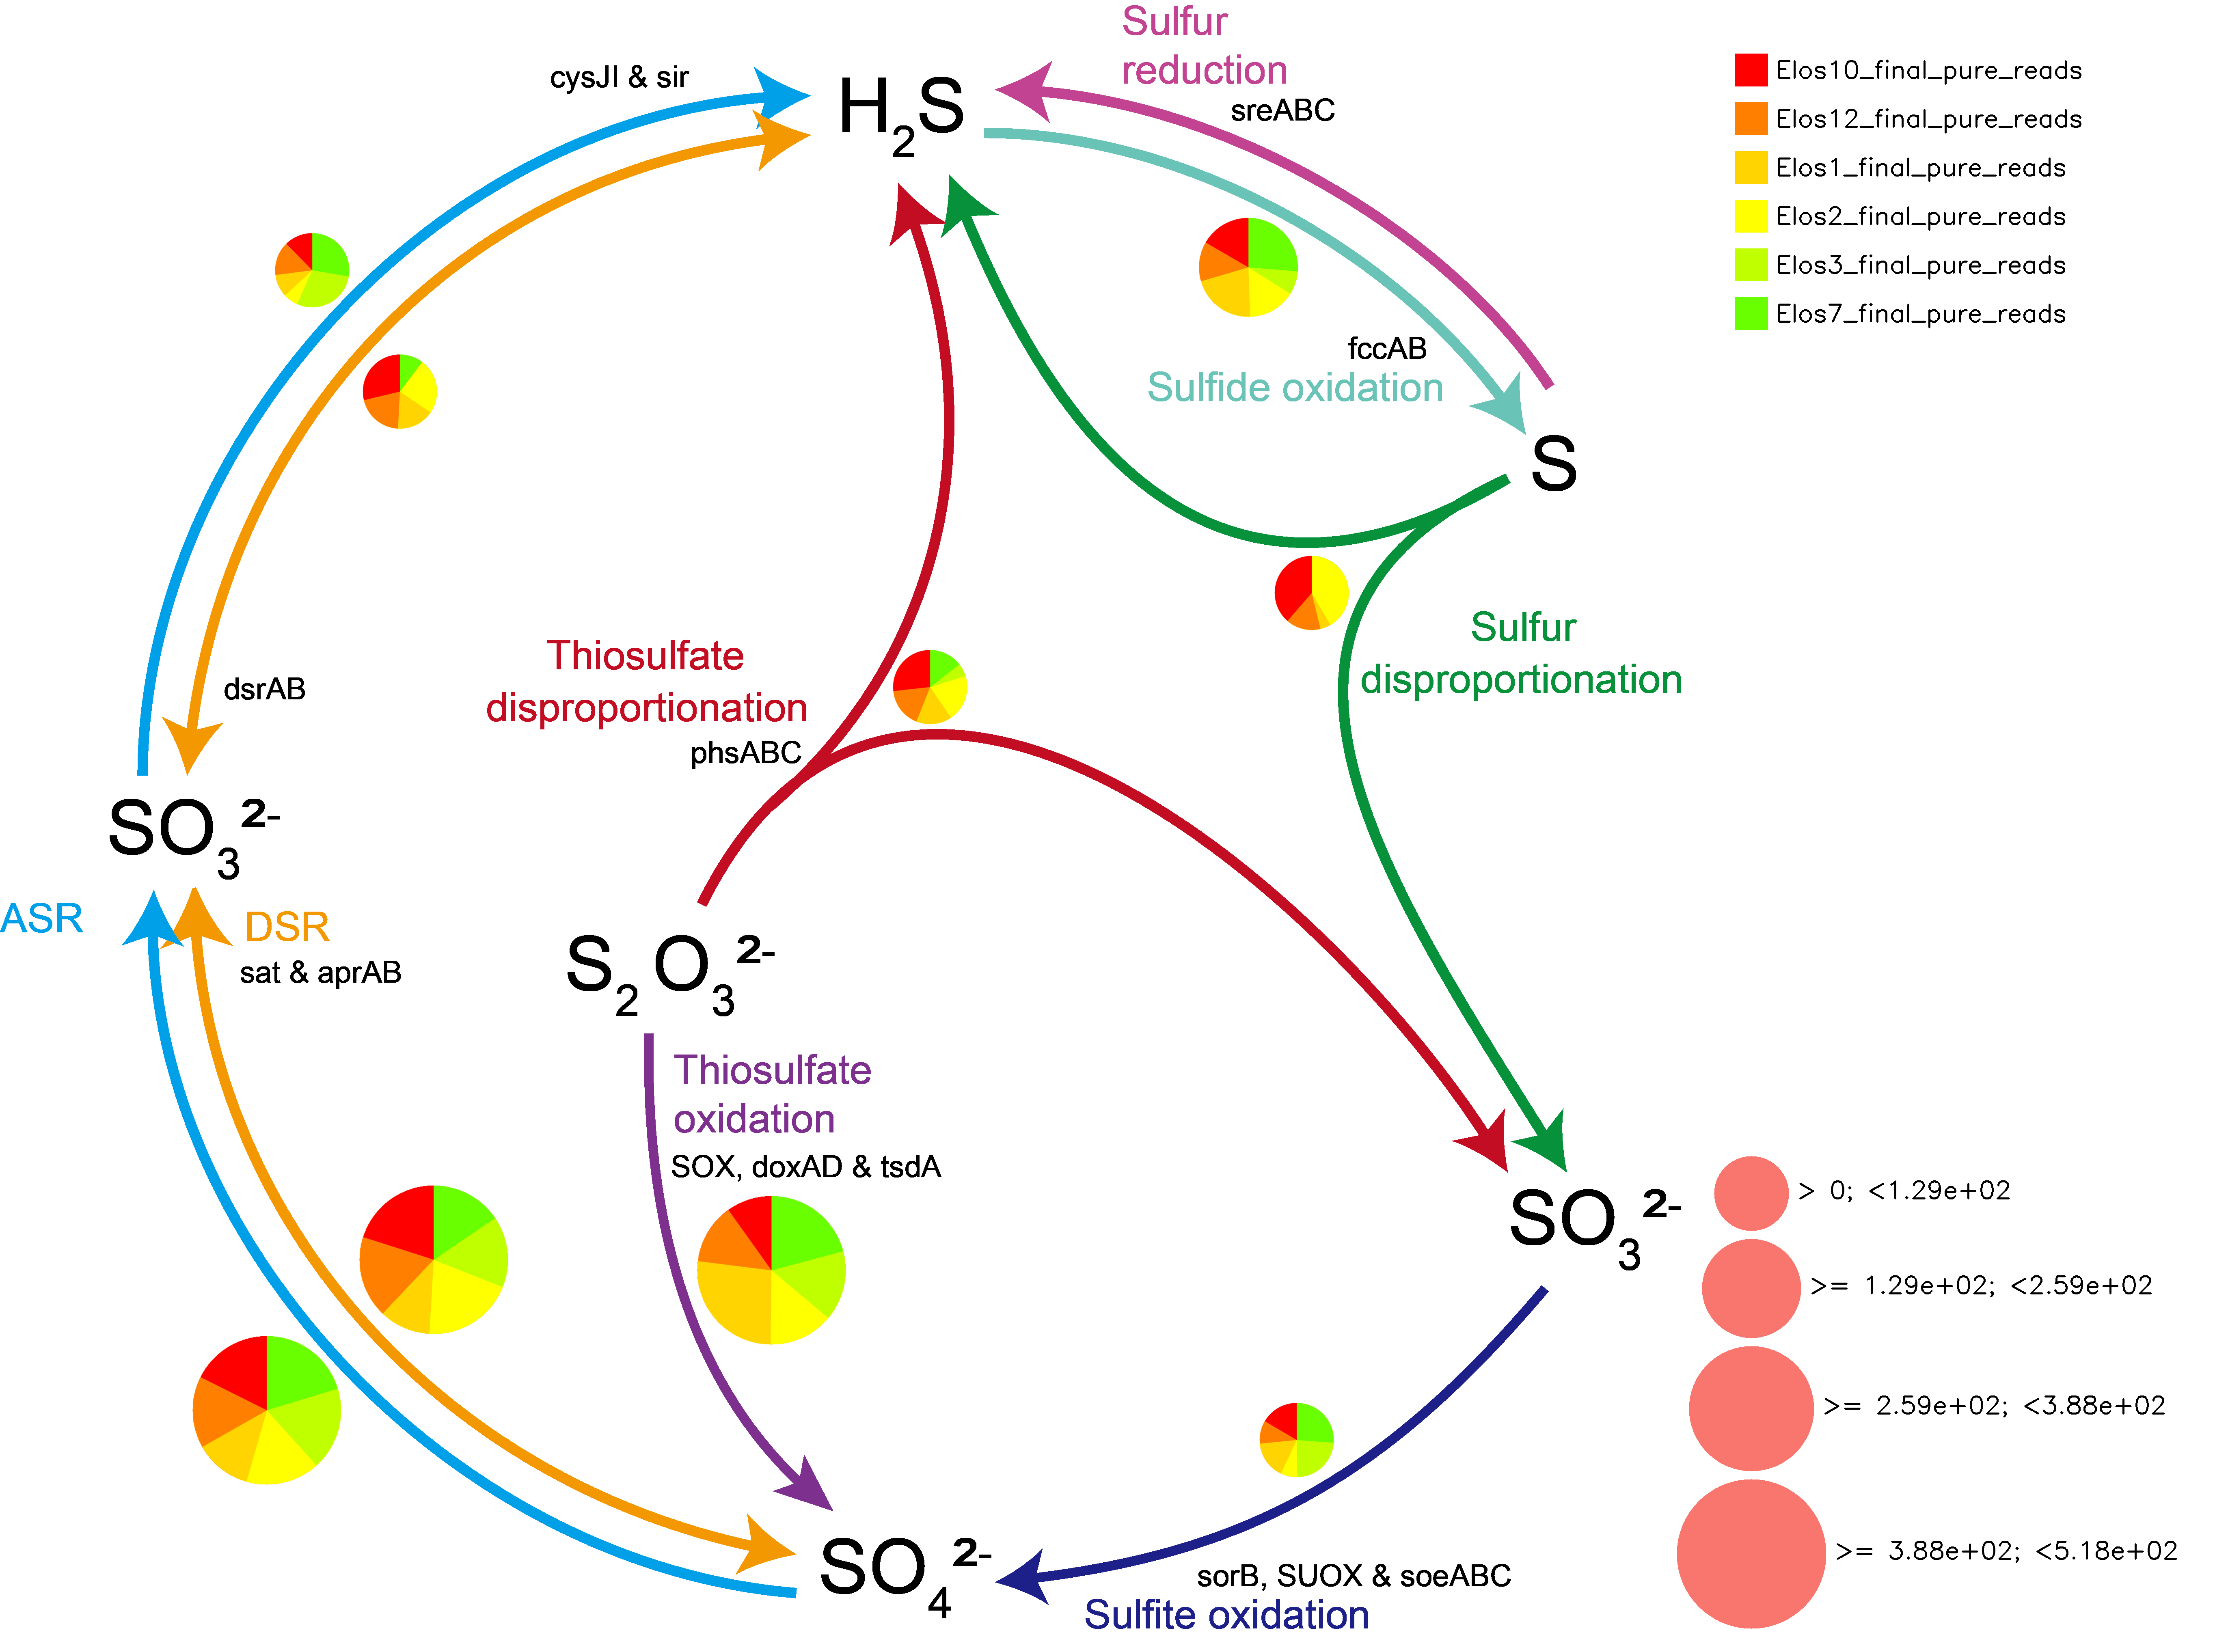
\includegraphics[width=0.98\columnwidth]{figures/sulfur_cycle_karpathos.png}
      \caption[Relative abundances of the pathways involved in the sulphur cycle]{
         Relative abundances of the pathways involved in the sulphur cycle. 
         The pie chart indicates the relative abundance of each pathway in each sample. 
         The size of pie charts represent the total relative abundance of each pathway. 
         ASR: assimilatory sulphate reduction; DSR: dissimilatory sulphate reduction.
      }
      \label{fig:karpathos-sulfur}
   \end{figure}   


   \begin{figure}[!htbp]
      \centering
      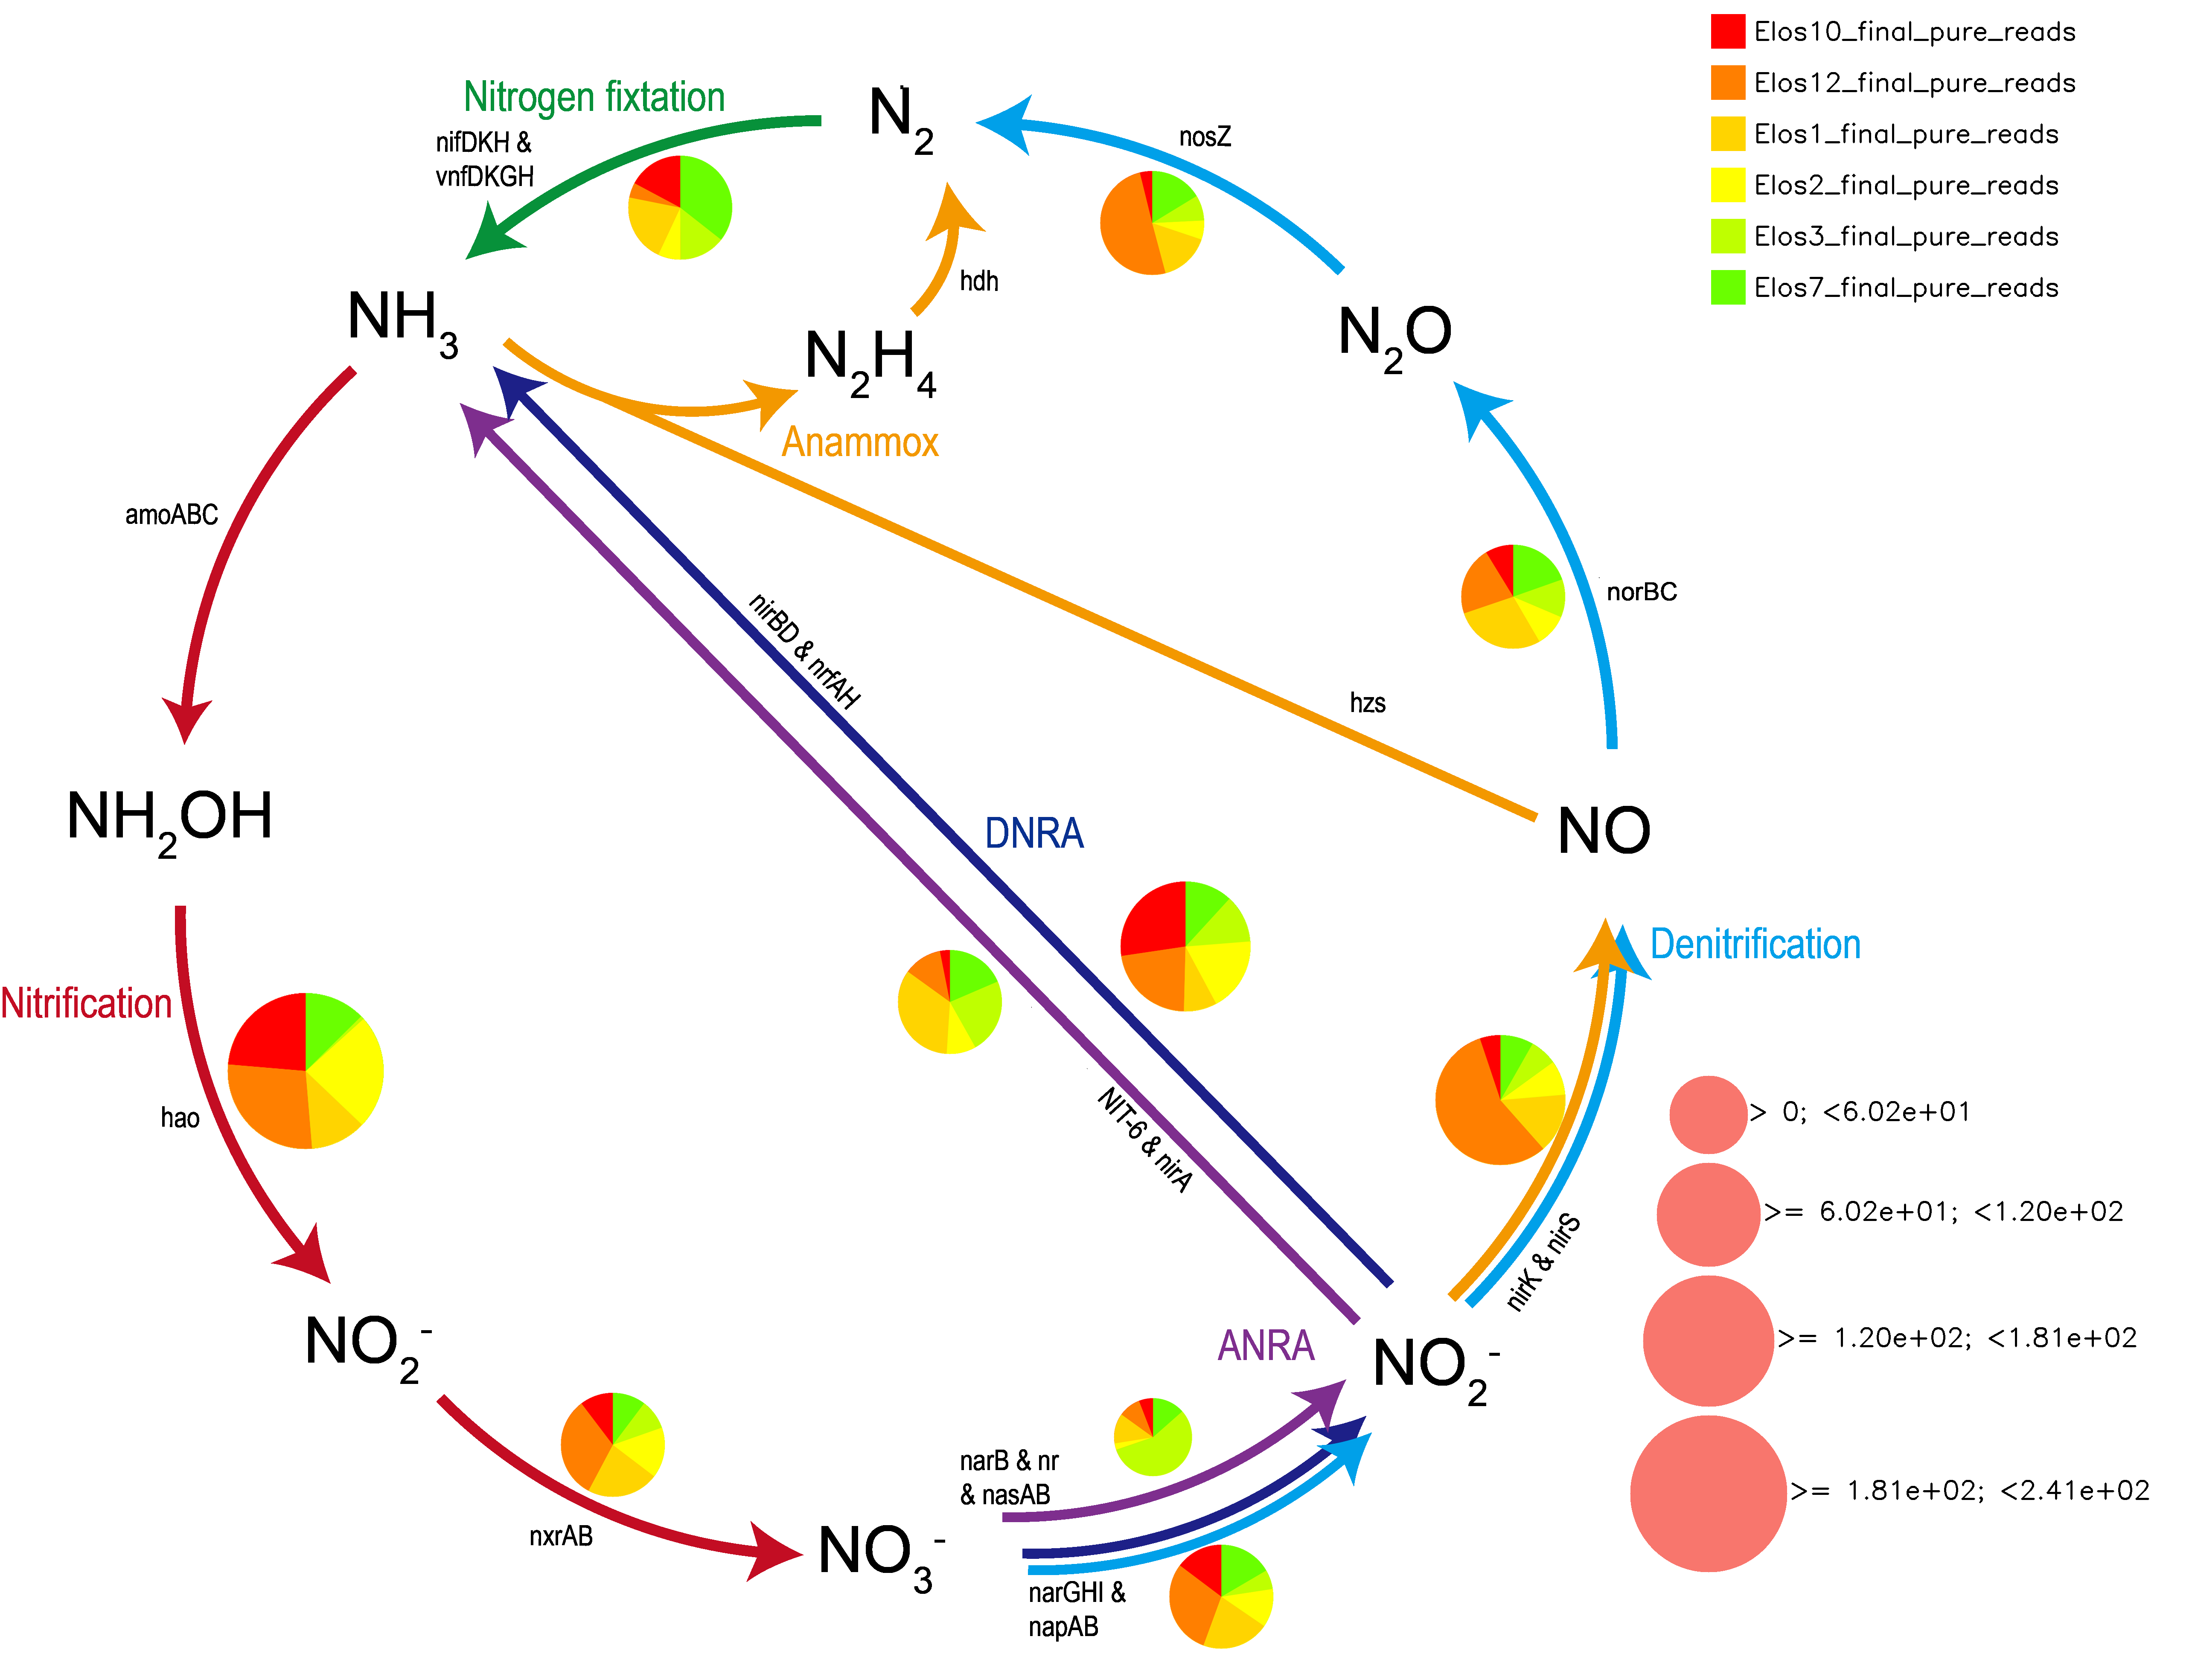
\includegraphics[width=0.98\columnwidth]{figures/nitrogen_cycle_karpathos.png}
      \caption[Relative abundances of the pathways involved in the nitrogen cycle]{
         Relative abundances of the pathways involved in the nitrogen cycle. 
         The pie chart indicates the relative abundance of each pathway in each sample. 
         The size of pie charts represent the total relative abundance of each pathway. 
         ANRA: assimilatory nitrate reduction to ammonium; 
         DNRA: dissimilatory nitrate reduction to ammonium; 
         Anammox: anaerobic ammonium oxidation. 
      }
      \label{fig:karpathos-nitrogen}
   \end{figure}   


% AFOULOPAPER DISCUSSION
\subsection{Discussion}
\label{swamp:discussion}

   Overall, there seems to be an agreement in all three ways that taxonomic composition has been derived for our samples. 
   Despite the fact that six out of the eleven samples were sequenced using shotgun metagenomics, 
   still we can compare them with the amplicon data and derive conclusions. In fact, the amplicon survey produced results 
   that were highly correlated to the results of the classification of the retrieved bins; 
   such congruence between the two methodologies has been reported in recent studies 
   \citep{chan_diversity_2015, regalado_combining_2020}
   although there is also evidence for the opposite~\citep{tessler_large-scale_2017}. 
   The results from Kraken2 were also correlated to the amplicon and the results of the classification of the retrieved MAGs, 
   although the correlation was not as strong. 
   However, Kraken2 is not restricted in the short amplicon length~\citep{johnson_evaluation_2019} 
   and therefore it was able to reach species level resolution~\citep{lu_ultrafast_2020}.

   The top sediment layer, i.e. the microbial mat, was characterised by the presence of Halobacteria/Halobacteriota, 
   Halanaerobiia and Nanoarchaeota which are all halophilic and were therefore able to withstand the salt crust that was on top of the mat 
   \citep{norton_archaeal_1993, casanueva_nanoarchaeal_2008, cinar_prokaryotic_2020, akpolat_prokaryotic_2021}
   They are almost absent in the deeper sediment layers and they are absent in the winter, 
   when there was no obvious microbial mat formed, despite the high salinity in sample Elos12. 
   Therefore, the limiting factor for their presence could have been the lower temperature during the winter season, 
   since the optimum temperature for representatives of the Halobacteria is higher than 35°C~\citep{grant_halobacterium_2015}. 
   Halobacteria, and their bacteriorhodopsin, are most likely responsible for the purple layer in the microbial mat, 
   since they have been shown to cause striking red colours in salt flats~\citep{stoeckenius_bacteriorhodopsin_1979}. 
   Nanoarchaeota are obligate symbionts and they have found in association with Crenarchaeota/Thermoproteota 
   \citep{huber_new_2002, podar_insights_2013, munson-mcgee_nanoarchaeota_2015, wurch_genomics-informed_2016, merkel_microbial_2017}.
   Out of the known host-symbiont pairs and the putative hosts that have been proposed, we identified two of the known hosts 
   (\textit{Ignicoccus hospitalis} and \textit{Acidilobus} sp. 7A) 
   and five of the putative hosts \citep{jarett_single-cell_2018}. 
   However, the Nanoarchaeotal representatives were assigned at taxonomies higher than the species level. 
   Thus, we can only presume that the symbionts \textit{Nanoarchaeum equitans} and \textit{Nanopusillus acidilobi} 
   of the aforementioned hosts are present in our data. 

   It was hypothesised that the microbial aggregates would be more closely related to the microbial mat samples 
   and this was confirmed by our results. 
   However, the microbial aggregates were mostly characterised by the presence of Bacteroidetes/Bacteroidota and Myxococcota 
   and the absence, or very low abundance, of Desulfobacterota, Thermoplasmatota and Asgardarchaeota.

   In the photic zone of the microbial mats, phototrophic microorganisms transduce light into energy 
   using either pigments 
   (chlorophyll and/or bacteriochlorophylls) or retinal-based rhodopsins~\citep{kurth_carbon_2021}. 
   In hypersaline microbial mats, phototrophy is possible because light can penetrate salt crusts and therefore 
   the only limiting factor is the capability of the microbial communities to actually perform 
   phototrophy under salt-saturated conditions~\citep{meier_limitation_2021}. 
   Out of the phyla that have been reported to perform (bacterio)chlorophyll-based phototrophy, 
   i.e. Cyanobacteria, Proteobacteria, Chlorobi/Chlorobia, Chloroflexi/Chloroflexota, Firmicutes, Acidobacteria/Acidobacteriota, 
   Eremiobacterota and Gemmatimonadetes/Gemmatimonadota (Zeng and Koblížek 2017; Zheng et al. 2022), 
   only Proteobacteria and Chloroflexi/Chloroflexota were found in high abundances. 
   Cyanobacteria were very rare in our samples, which can be attributed to the high salinity of the marsh~\citep{diloreto_microbial_2019} 
   which can lead to osmotic stress and inhibition of photosynthesis~\citep{sudhir_effects_2004}. 
   So, Cyanobacteria were not the foundation of the microbial mats in our study, 
   as has been shown in other examples of hypersaline microbial mats 
   \citep{bolhuis_molecular_2014, wong_molecular_2016}, 
   which was expected as oxygenic photosynthesis is completely inhibited at saturation-level salinities (40\%)~\citep{meier_limitation_2021}. 
   However, cyanobacterial genera that  are characterised by strategies and survival mechanisms 
   that allow them to grow in such high salinities~\citep{oren_cyanobacteria_2015}, 
   such as \textit{Euhalothece} and \textit{Halothece}, were present in our samples. 
   Chloroflexi/Chloroflexota were most present in the bottom sediment layer and in the combined sediment samples. 
   Representatives that were identified from our samples are Chloroflexus aurantiacus~\citep{pierson_phototrophic_1974}
   and \textit{C. aggregans}~\citep{hanada_chloroflexus_1995}; 
   they can grow photoautotrophically and photoheterotrophically 
   under anaerobic conditions but also chemotrophically under aerobic conditions, 
   using sulphide or hydrogen as an electron donor~\citep{tang_complete_2011, kawai_hydrogen-dependent_2019, kawai_-situ_2021}. 
   Given that it is unclear if they can harvest light deeper in the sediment and taking into account 
   the low abundance of Cyanobacteria, it is most probable that Chloroflexi/Chloroflexota grow chemotrophically in our samples. 
   According to our data, Proteobacteria seem to be taking over the photosynthetic pathways in our samples. 
   More specifically, some of the species that have been found to perform photosynthesis and are present in our samples are
   (from the Alphaproteobacteria class) \textit{Citromicrobium} sp.~\citep{jiao_coexistence_2010}, 
   \textit{Rhodopseudomonas palustris}, \textit{Rhodobacter} sp., \textit{Rhodospirillum rubrum}, 
   \textit{Roseobacter denitrificans}, \textit{Bradyrhizobium} sp., \textit{Roseobacter} sp. 
   \citep{larimer_complete_2004, bryant_prokaryotic_2006}
   and (from the Gammaproteobacteria class) 
   \textit{Marichromatium purpuratum}~\citep{shiung_photosynthetic_2018}, 
   \textit{Congregibacter litoralis}~\citep{fuchs_characterization_2007, spring_photosynthetic_2009}, 
   \textit{Allochromatium} spp.~\citep{kyndt_genome_2020}. 
   Overall, based on the taxonomic composition of the studied microbial mats, 
   it seems that they resemble microbial mats from an irregularly inundated tidal flat in Oman~\citep{meier_limitation_2021}.


   Our second hypothesis was that samples from the deeper sediment layers collected in the summer would be more similar to 
   the combined sediment samples collected in the winter. 
   This was also confirmed by our results, as these samples were clustered together. 
   However, despite the similarities between the samples, there were also certain differences; 
   as expected, there is a high degree of spatial variation in the marsh under study~\citep{dillon_spatial_2009}. 
   Overall, in the deeper sediment layers or where microbial mat was not formed, acetogens such as 
   \textit{Moorella thermoacetica}, \textit{Clostridium aceticum} and \textit{Acetobacterium woodii}~\citep{schuchmann_energetics_2016}, 
   were utilising the Wood–Ljungdahl pathway, i.e. using H2 hydrogen as an electron donor and CO2 as an electron acceptor. 
   Acetogens are either competing directly with hydrogenotrophic methanogenic archaea or interacting syntrophically 
   with acetotrophic methanogens~\citep{ragsdale_acetogenesis_2008}. 
   Utilisation of acetate for methanogenesis is present in the genera \textit{Methanosarcina} and \textit{Methanothrix} (Ferry 1992) 
   which are both found in our samples. 
   Although while abundant in our samples, methanogens might have been contributing little to anaerobic mineralization, 
   since in salinities of 180‰ or less they are inhibited by the increased activity of sulphate-reducing bacteria 
   \citep{sorensen_salinity_2004}. 
   In addition, sulphate-reducing bacteria might have also been using the Wood-Ljungdahl pathway in reverse 
   \citep{ragsdale_acetogenesis_2008}. 
   Sulphate-reducing microorganisms (SRM) from the Euryarchaeota lineage~\citep{muyzer_ecology_2008} were very abundant 
   in the microbial mat and in the aggregates, while SRM belonging to Deltaproteobacteria~\citep{muyzer_ecology_2008} 
   are present  in the deeper and the combined sediment samples. 
   However, the occurrence of SRMs is not synonymous to the occurrence of sulphate reduction in the given habitat~\citep{muyzer_ecology_2008}.

   It has been proposed that arsenic and sulphur cycling can sustain high microbial metabolic rates in permanently anoxic mats~\citep{visscher_modern_2020}. 
   Bacteria capable of performing anoxygenic photosynthesis using arsenite (As(III)) as an electron donor, 
   such as \textit{Ectothiorhodospira} sp. and \textit{Halorhodospira halophila}~\citep{hoeft_mccann_arsenite_2017}, are present in our samples. 
   It is suggested that they are performing oxidation of As(III) to arsenate (As(V)), which is afterwards reduced back to As(III) (Hoeft et al. 2004), 
   thus explaining the high occurrence of dissimilatory arsenic reduction in our samples. 
   Arsenate can be an important electron acceptor in the biogeochemical cycling of carbon~\citep{oremland_bacterial_2000}; 
   thus, arsenate reduction has a great potential to precipitate carbonates and it is energetically better than sulphate reduction~\citep{visscher_modern_2020}, 
   although the latter is also very abundant in our samples. 
   Thaumarchaeota, which are involved in nitrification in marine ecosystems~\citep{veuger_nitrification_2013}, 
   were also present in our samples but in very low abundances, in contrast to other hypersaline microbial mats~\citep{ruvindy_unravelling_2016}. 
   On the other hand, common nitrifying bacteria such as \textit{Nitrobacter} where abundant in our samples; 
   however, since nitrification was mostly present in the combined sediments and in the deeper layer, 
   there seems to be a certain degree of hypersalinity limitation on the growth of nitrifying bacteria, 
   as has been previously suggested~\citep{jeffries_increases_2012}. 
   Denitrification was also present in our samples, although mostly in the combined sediment, and it was not limited by 
   the increased salinity~\citep{laverman_potential_2007}. 
   Regarding functional annotation of MAGs and their clustering according to taxonomy, 
   it seems that it is driven by modules that are present in Archaea and absent in Bacteria, and vice versa. 
   For example, regarding cysteine biosynthesis (M00021), this pathway is still unexplored in Archaea 
   and although it has been found in certain species, e.g. \textit{Methanosarcina barkeri}, 
   it is suggested that there might be a different cysteine biosynthesis pathway in Archaea~\citep*{kitabatake_cysteine_2000}. 
   Likewise, there are no archaeal homologs for the bacterial pantothenate biosynthetic genes~\citep{ronconi_novel_2008}, 
   therefore pantothenate biosynthesis (M00913) is one of the pathways that contributes 
   to the differentiation between bacterial and archaeal MAGs. 
   In addition, acetogen (M00618) is only found in Bacteria.
   
   It has been debated if hypersaline environments are thermodynamic limiting the occurrence of self-sustaining 
   microbial communities~\citep{oren_thermodynamic_2011} or if they are biologically permissive~\citep{lee_nacl-saturated_2018}. 
   Cells need to implement strategies to counteract the osmotic stress~\citep{gunde-cimerman_strategies_2018} 
   but these strategies come with an energetic cost~\citep{meier_limitation_2021}. 
   It has been suggested that hypersaline microbial mats and, in particular, communities below salt crusts, 
   cannot rely solely on primary production from anoxygenic phototrophy and mineralization from sulphate reduction~\citep{meier_limitation_2021}. 
   Instead, import of reduced substances and periods of reduced salinity are required, 
   to allow the occurrence of oxygenic photosynthesis~\citep{meier_limitation_2021}; 
   in our study site this occurs in winter where evaporation is not as strong as in the summer, 
   which combined with the increased precipitation, lowers the salinity of the marsh. 
   During winter months, both the salt crust and the layering of the microbial mat disappears, as in \cite{cardoso_seasonal_2019}, 
   and it seems that this temporal change and seasonal development of the microbial mats under study is the necessary element for the survival of the microorganisms. 
   In addition, anaplerotic reactions, that are abundant in our samples, may play an important role in replenishing the intermediates of the TCA cycle, 
   which is quite abundant in out samples, and thus allowing microbial growth with a carbohydrate 
   as the sole carbon source~\citep{tong_structure_2013, choi_distinct_2016}. 
   Although it seems that hypersaline environments are “thermodynamically moderate”, DNA based studies can only identify 
   the members of a community and not their metabolic activities. 
   Therefore future studies on hypersaline microbial mats should focus on the combination of metabolomics, 
   metatranscriptomics and metagenomics, in order to elucidate the functional repertoire of microbial communities, 
   their metabolic potential and their metabolic and ecological interactions. 
   Metabolic modelling of the microbial assemblages can shed further light on the effects of the environmental 
   challenges on the mat construction as well as on which processes are taking place within each mat layer and 
   among its different layers.


\subsection*{Supplementary Material}
\label{swamp:suppl}   

   The Supplementary Material for this study will be publically available once it is published. 
   For the time being, they can be found under this \href{https://drive.google.com/drive/folders/1eQiXxsUPJ4QuIFxa1g5dWFw0CySuYvKD?usp=sharing}{Google Drive folder}.

   \textbf{Supplementary Figure 1:} nMDS of the similarity matrix of the samples based on the microbial OTUs relative abundances, as retrieved from the amplicon sequencing. 

   \textbf{Supplementary Figure 2:} Bar chart showing the abundances of the main microbial taxa, at the phylum level, at each sample, as retrieved from Kraken2. 

   \textbf{Supplementary Figure 3:} Blobology scatterplot showing the contigs that were binned (blue) and the contigs that were not binned (grey). 

   \textbf{Supplementary Figure 4:} Blobology scatterplot showing the contigs that were binned and their taxonomic annotation. blue: Bacteria; yellow: Archaea; red: Eukaryota; grey: not assigned. 

   \textbf{Supplementary Figure 5:} Bar chart showing the abundances of the main microbial taxa, at the phylum level, at each sample, as retrieved from the classification of the retrieved MAGs.

   \textbf{Supplementary Figure 6:} \texttt{MetaWRAP} heatmap showing the similarity and clustering of the samples based on the identified bins.  

   \textbf{Supplementary Figure 7:} Distribution of the number of KO terms annotated per MAG. 

   \textbf{Supplementary Figure 8:} Distribution of the number of the complete KEGG modules present per MAG. 

   \textbf{Supplementary Figure 9:} nMDS of the similarity matrix of the MAGs based on the presence/absence of their modules. 

   \textbf{Supplementary Figure 10:} Relative abundances of the pathways involved in the carbon cycle. The pie chart indicates the relative abundance of each pathway in each sample. The size of pie charts represent the total relative abundance of each pathway. 
                                    CBB: Calvin-Benson-Bassham cycle; rTCA: reductive citric acid cycle; WL: Wood-Ljungdahl pathway; 3HB: 3-hydroxypropionate bicycle; DHC: Dicarboxylate-hydroxybutyrate cycle.

   \textbf{Supplementary Figure 11:} Relative abundances of the pathways involved in the DMSP cycle. The pie chart indicates the relative abundance of each pathway in each sample. The size of pie charts represent the total relative abundance of each pathway. 
    
   \textbf{Supplementary File 1:} The parameters for the PEMA processing of the 16S rRNA amplicon data.
    
   \textbf{Supplementary File 2:} Details of the MAGs’ processing. 
   


\subsection*{MAGs description}

   In Appendix~\ref{app:mags} the methodology for the description of the reconstructed MAGs 
   from the Tristomo marsh data can be found. 
   The novel taxa found will be thoroughly investigated in the near future. 


%%% Local Variables: 
%%% mode: latex
%%% TeX-master: "thesis"
%%% End: 
